\section{Experiments}
\label{sec:experiments}

\begin{figure}[!t]
	\centering
	
\includegraphics[width=0.42\textwidth]{figures/data.png}
	\caption{Geographical visualization of the two wind farm datasets used in the experiments.}
	\label{fig:dataset_geography}
\end{figure}

\begin{table*}[!t]
	\caption{Detailed full-sample forecasting performance on the Penmanshiel dataset under the noise-free setting. Lower values indicate better performance.}
	\label{tab:main_penmanshiel}
	\centering
	\scriptsize
	\setlength{\tabcolsep}{5pt}
	\renewcommand{\arraystretch}{1.04}
	\begin{adjustbox}{max width=\textwidth}
		\begin{tabular}{llcccccccc}
			\toprule
			Metric & Horizon & WindFormer & MST-Net & TimeMixer++ & iTransformer & PatchTST & TimesNet & GLPT & DLinear \\
			\midrule
			\multirow{3}{*}{Speed MAE} & 6 & \textbf{0.7142} & 0.7978 & 0.9229 & 0.9272 & 0.9189 & 0.9210 & 0.9318 & 0.9263 \\
			& 12 & \textbf{0.8812} & 0.9879 & 1.1421 & 1.1491 & 1.1347 & 1.1406 & 1.1543 & 1.1473 \\
			& 18 & \textbf{1.0103} & 1.1249 & 1.2994 & 1.3081 & 1.2891 & 1.2976 & 1.3138 & 1.3061 \\
			\midrule
			\multirow{3}{*}{Speed RMSE} & 6 & \textbf{1.1497} & 1.2162 & 1.3053 & 1.3118 & 1.2987 & 1.3033 & 1.3174 & 1.3108 \\
			& 12 & \textbf{1.4211} & 1.5538 & 1.6162 & 1.6247 & 1.6054 & 1.6142 & 1.6325 & 1.6224 \\
			& 18 & \textbf{1.6216} & 1.7599 & 1.8367 & 1.8477 & 1.8263 & 1.8348 & 1.8553 & 1.8447 \\
			\midrule
			\multirow{3}{*}{Direction MAE} & 6 & \textbf{0.1456} & 0.1637 & 0.1898 & 0.1911 & 0.1884 & 0.1894 & 0.1926 & 0.1939 \\
			& 12 & \textbf{0.1881} & 0.2113 & 0.2439 & 0.2460 & 0.2403 & 0.2434 & 0.2483 & 0.2497 \\
			& 18 & \textbf{0.2204} & 0.2471 & 0.2847 & 0.2872 & 0.2807 & 0.2840 & 0.2899 & 0.2913 \\
			\midrule
			\multirow{3}{*}{Direction RMSE} & 6 & \textbf{0.2914} & 0.3092 & 0.3314 & 0.3341 & 0.3294 & 0.3320 & 0.3354 & 0.3375 \\
			& 12 & \textbf{0.3686} & 0.3905 & 0.4176 & 0.4213 & 0.4146 & 0.4184 & 0.4237 & 0.4260 \\
			& 18 & \textbf{0.4244} & 0.4599 & 0.4796 & 0.4843 & 0.4761 & 0.4807 & 0.4870 & 0.4906 \\
			\bottomrule
		\end{tabular}
	\end{adjustbox}
\end{table*}

\subsection{Experimental Setup}
\label{subsec:experimental_setup}

We evaluate the model on two SCADA-based wind farm datasets with distinct spatial layouts and wind regimes: Shanxi with 24 turbines and Penmanshiel with 14 turbines. Both datasets are sampled at 10-min intervals and preprocessed following the protocol in Section~\ref{sec:data_preprocessing_task}. Unless otherwise specified, the input window is 288 steps, corresponding to 48 h of history, and the forecasting horizons are 6, 12, and 18 steps.



WindFormer is compared with MST-Net, PatchTST, TimeMixer++, GLPT, DLinear, TimesNet, and iTransformer. MAE and RMSE are reported for wind speed (m/s) and wind direction (rad). Beyond the full-sample benchmark, robustness and sparse-deployment generalization are further evaluated.

\subsection{Standard Forecasting Evaluation}
\label{subsec:standard_forecasting}

The standard setting trains and tests on the full turbine set without artificial perturbation.



\begin{table*}[!t]
\caption{Detailed full-sample forecasting performance on the Shanxi dataset under the noise-free setting. Lower values indicate better performance.}
\label{tab:main_shanxi}
\centering
\scriptsize
\setlength{\tabcolsep}{5pt}
\renewcommand{\arraystretch}{1.04}
\begin{adjustbox}{max width=\textwidth}
\begin{tabular}{llcccccccc}
\toprule
			Metric & Horizon & WindFormer & MST-Net & TimeMixer++ & iTransformer & PatchTST & TimesNet & GLPT & DLinear \\
\midrule
\multirow{3}{*}{Speed MAE} & 6 & \textbf{0.6367} & 0.7062 & 0.8192 & 0.8222 & 0.8165 & 0.8274 & 0.8270 & 0.8217 \\
 & 12 & \textbf{0.8025} & 0.8939 & 1.0343 & 1.0395 & 1.0309 & 1.0452 & 1.0447 & 1.0379 \\
 & 18 & \textbf{0.9309} & 1.0337 & 1.1970 & 1.2024 & 1.1953 & 1.2098 & 1.2094 & 1.2013 \\
\midrule
\multirow{3}{*}{Speed RMSE} & 6 & \textbf{0.9884} & 1.0377 & 1.1203 & 1.1248 & 1.1172 & 1.1320 & 1.1311 & 1.1242 \\
 & 12 & \textbf{1.2374} & 1.3033 & 1.4035 & 1.4097 & 1.3986 & 1.4178 & 1.4167 & 1.4078 \\
 & 18 & \textbf{1.4116} & 1.4862 & 1.6002 & 1.6073 & 1.5987 & 1.6172 & 1.6161 & 1.6059 \\
\midrule
\multirow{3}{*}{Direction MAE} & 6 & \textbf{0.2717} & 0.2984 & 0.3460 & 0.3478 & 0.3445 & 0.3507 & 0.3500 & 0.3516 \\
 & 12 & \textbf{0.3441} & 0.3806 & 0.4403 & 0.4426 & 0.4384 & 0.4465 & 0.4459 & 0.4476 \\
 & 18 & \textbf{0.4019} & 0.4437 & 0.5130 & 0.5160 & 0.5115 & 0.5206 & 0.5199 & 0.5223 \\
\midrule
\multirow{3}{*}{Direction RMSE} & 6 & \textbf{0.5530} & 0.5778 & 0.6225 & 0.6269 & 0.6210 & 0.6283 & 0.6273 & 0.6300 \\
 & 12 & \textbf{0.6525} & 0.7041 & 0.7356 & 0.7409 & 0.7342 & 0.7454 & 0.7440 & 0.7471 \\
 & 18 & \textbf{0.7275} & 0.7831 & 0.8196 & 0.8255 & 0.8184 & 0.8295 & 0.8285 & 0.8324 \\
\bottomrule
\end{tabular}
\end{adjustbox}
\end{table*}

\begin{figure}[!t]
\centering
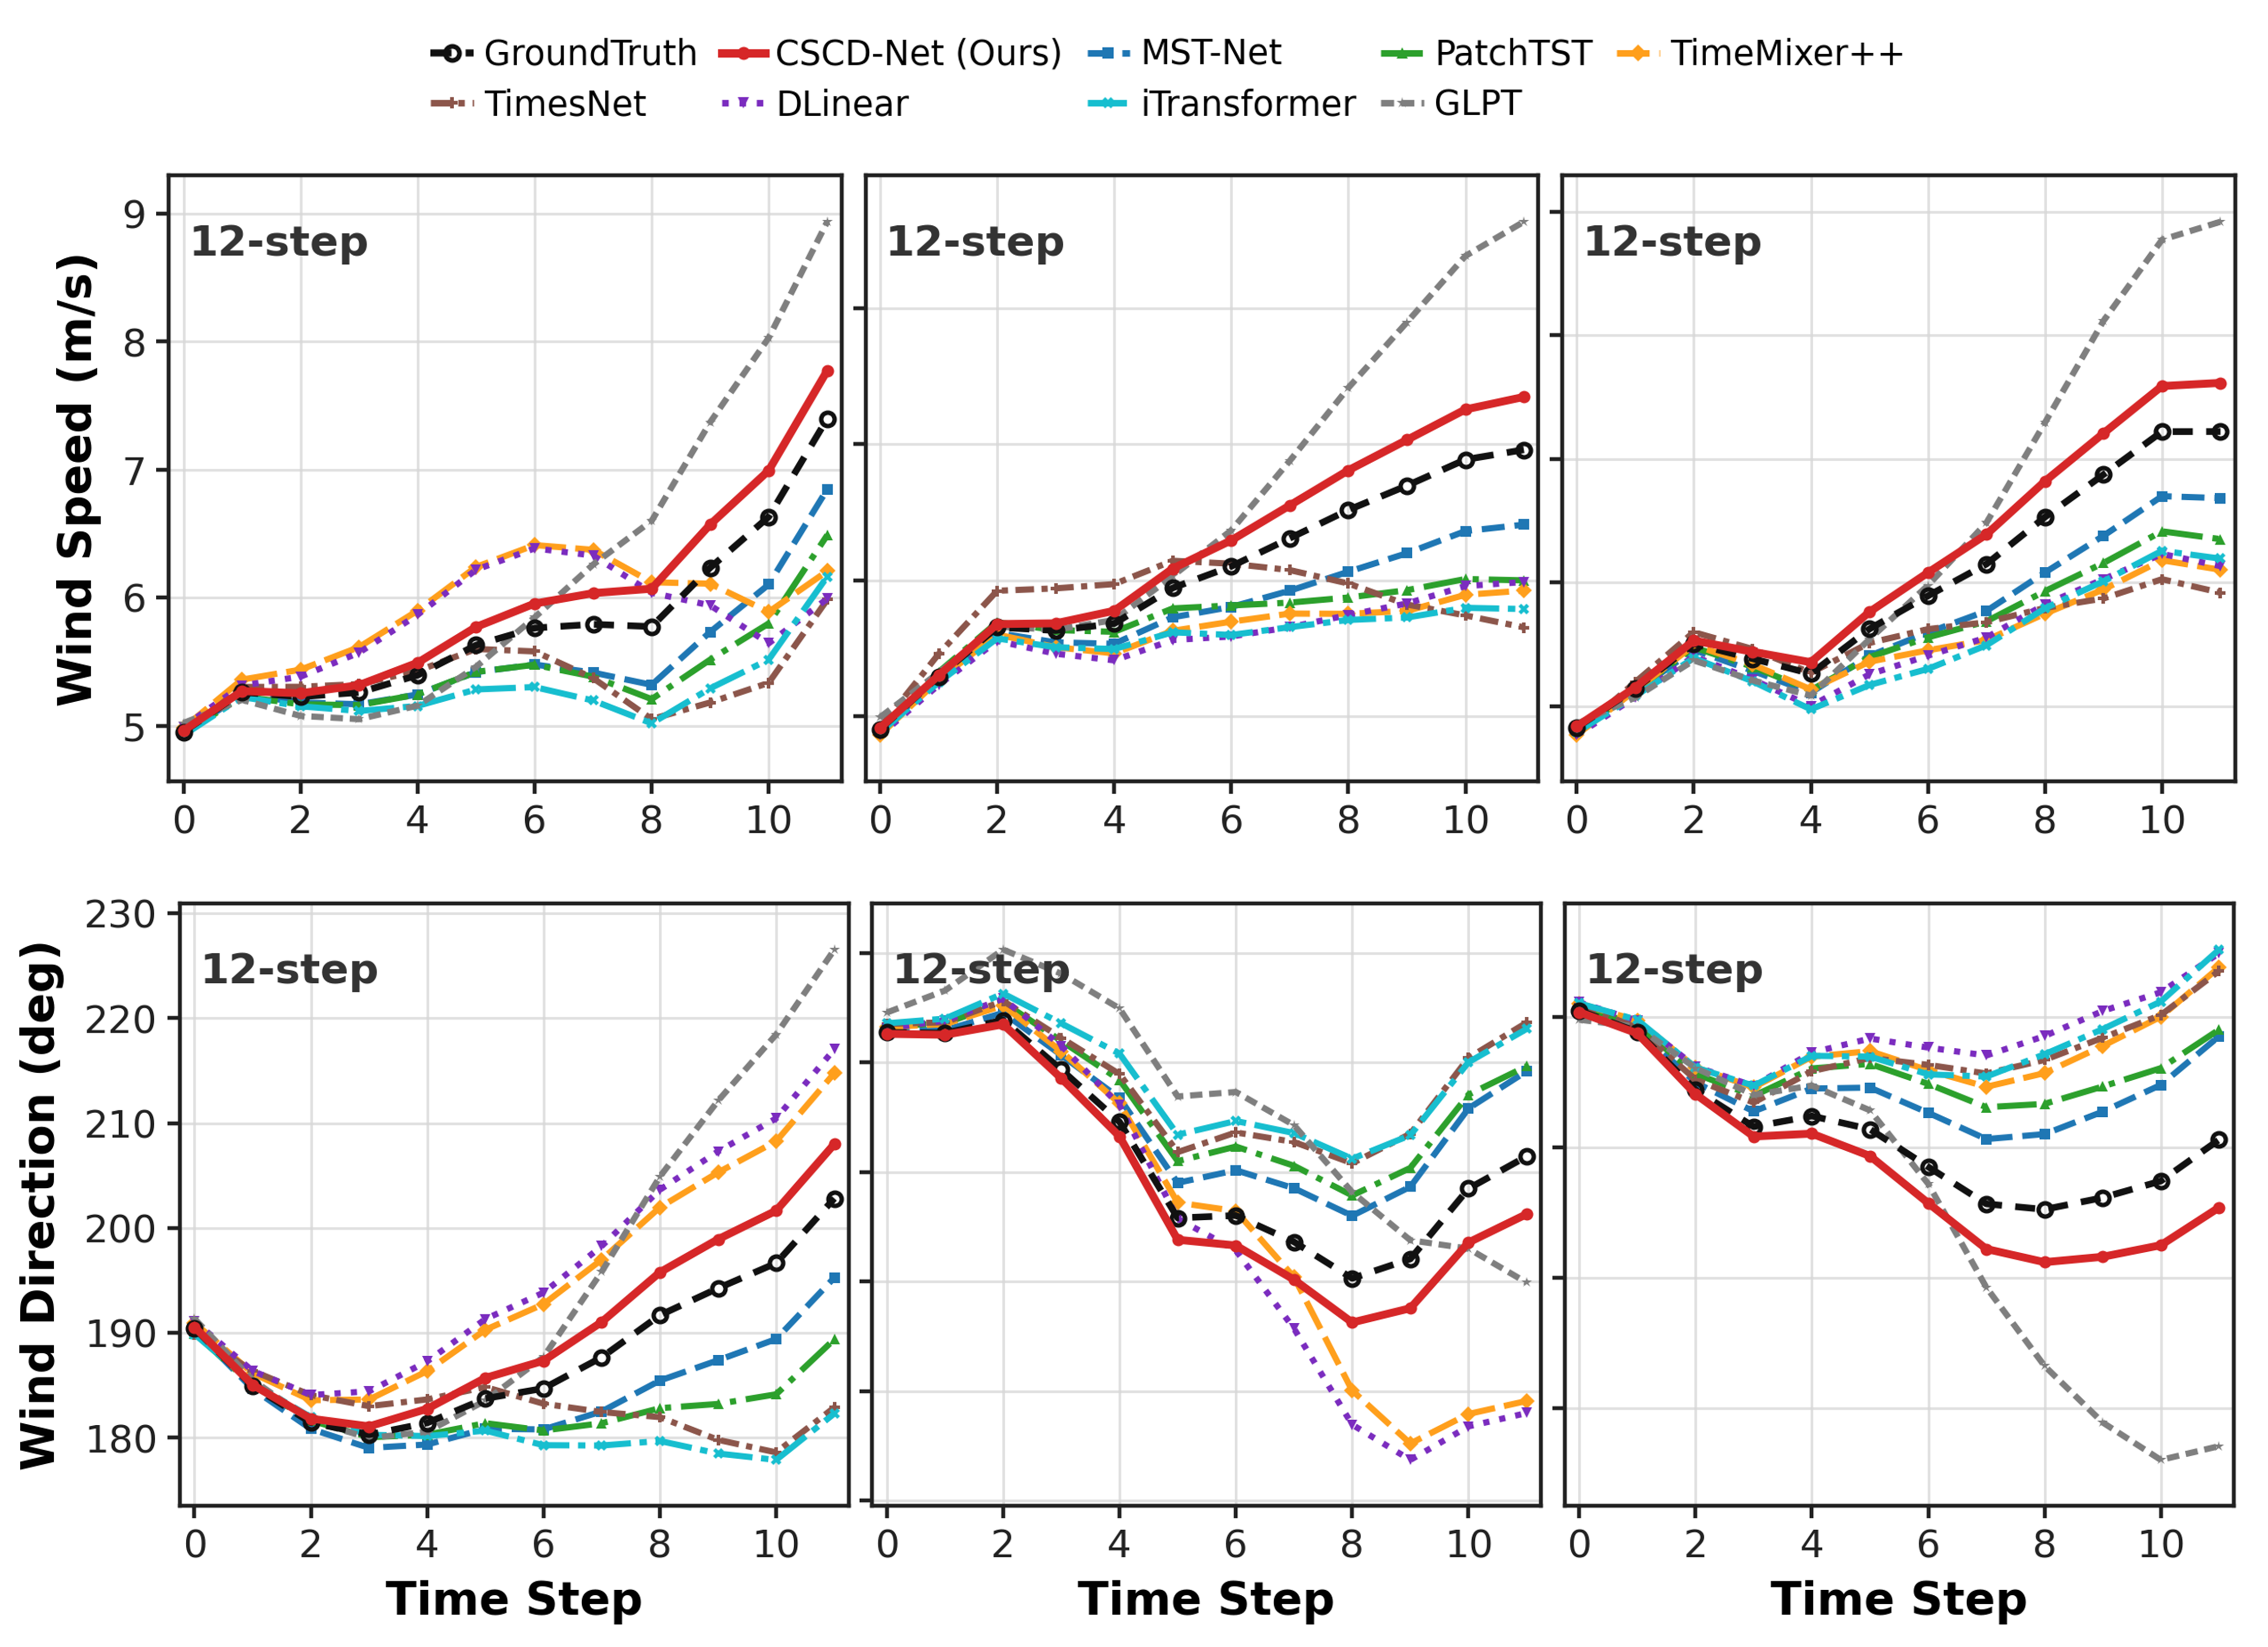
\includegraphics[width=0.48\textwidth]{figures/result.png}
\caption{Representative 12-step full-sample prediction examples for wind speed and wind direction.}
\label{fig:prediction_examples}
\end{figure}

Tables~\ref{tab:main_penmanshiel} and \ref{tab:main_shanxi} show that WindFormer achieves the best wind speed and wind direction accuracy across all horizons on both datasets.

\begin{table}[!t]
\caption{Computational efficiency comparison at the 12-step forecasting horizon.}
\label{tab:efficiency}
\centering
\scriptsize
\setlength{\tabcolsep}{2.0pt}
\renewcommand{\arraystretch}{1.04}
\begin{adjustbox}{max width=\columnwidth}
\begin{tabular}{@{}lccccc@{}}
\toprule
Metric & WindFormer & MSGNet & PatchTST & iTransformer & TimeMixer++ \\
\midrule
Parameters & 36,512 & 26,680,000 & 140,492 & 124,428 & 388,332 \\
Train time (s) & 143.78 & 14356.30 & 315.32 & 57.80 & 109.55 \\
Peak GPU (MB) & 74.83 & 4532.1 & 3158.9 & 109.1 & 308.9 \\
\bottomrule
\end{tabular}
\end{adjustbox}
\end{table}

Table~\ref{tab:efficiency} shows that WindFormer achieves competitive efficiency with 36,512 parameters and 74.83 MB peak GPU memory.

\subsection{Robustness Under Perturbation}
\label{subsec:robustness}

Two robustness experiments are designed: \emph{Sensor Perturbation Robustness} and \emph{Extreme Volatility Stress Test}. For sensor perturbation, let $\theta_{i,t}$ denote the wind direction of turbine $i$ at time $t$, and let $\mathcal{W}(\cdot)$ wrap angles to the valid range. Only the wind-direction channel in the training inputs is corrupted as
\begin{equation}
\tilde{\theta}_{i,t}^{(\sigma)}=\mathcal{W}\left(\theta_{i,t}+\epsilon_{i,t}^{(\sigma)}\right),\quad
\epsilon_{i,t}^{(\sigma)}\sim\mathcal{N}(0,\sigma^2),
\label{eq:sensor_noise}
\end{equation}
where $\sigma\in\{0.1,0.2,0.3\}$ rad. Test inputs and labels remain unchanged, and all models are retrained at each noise level.

\begin{figure}[!t]
\centering
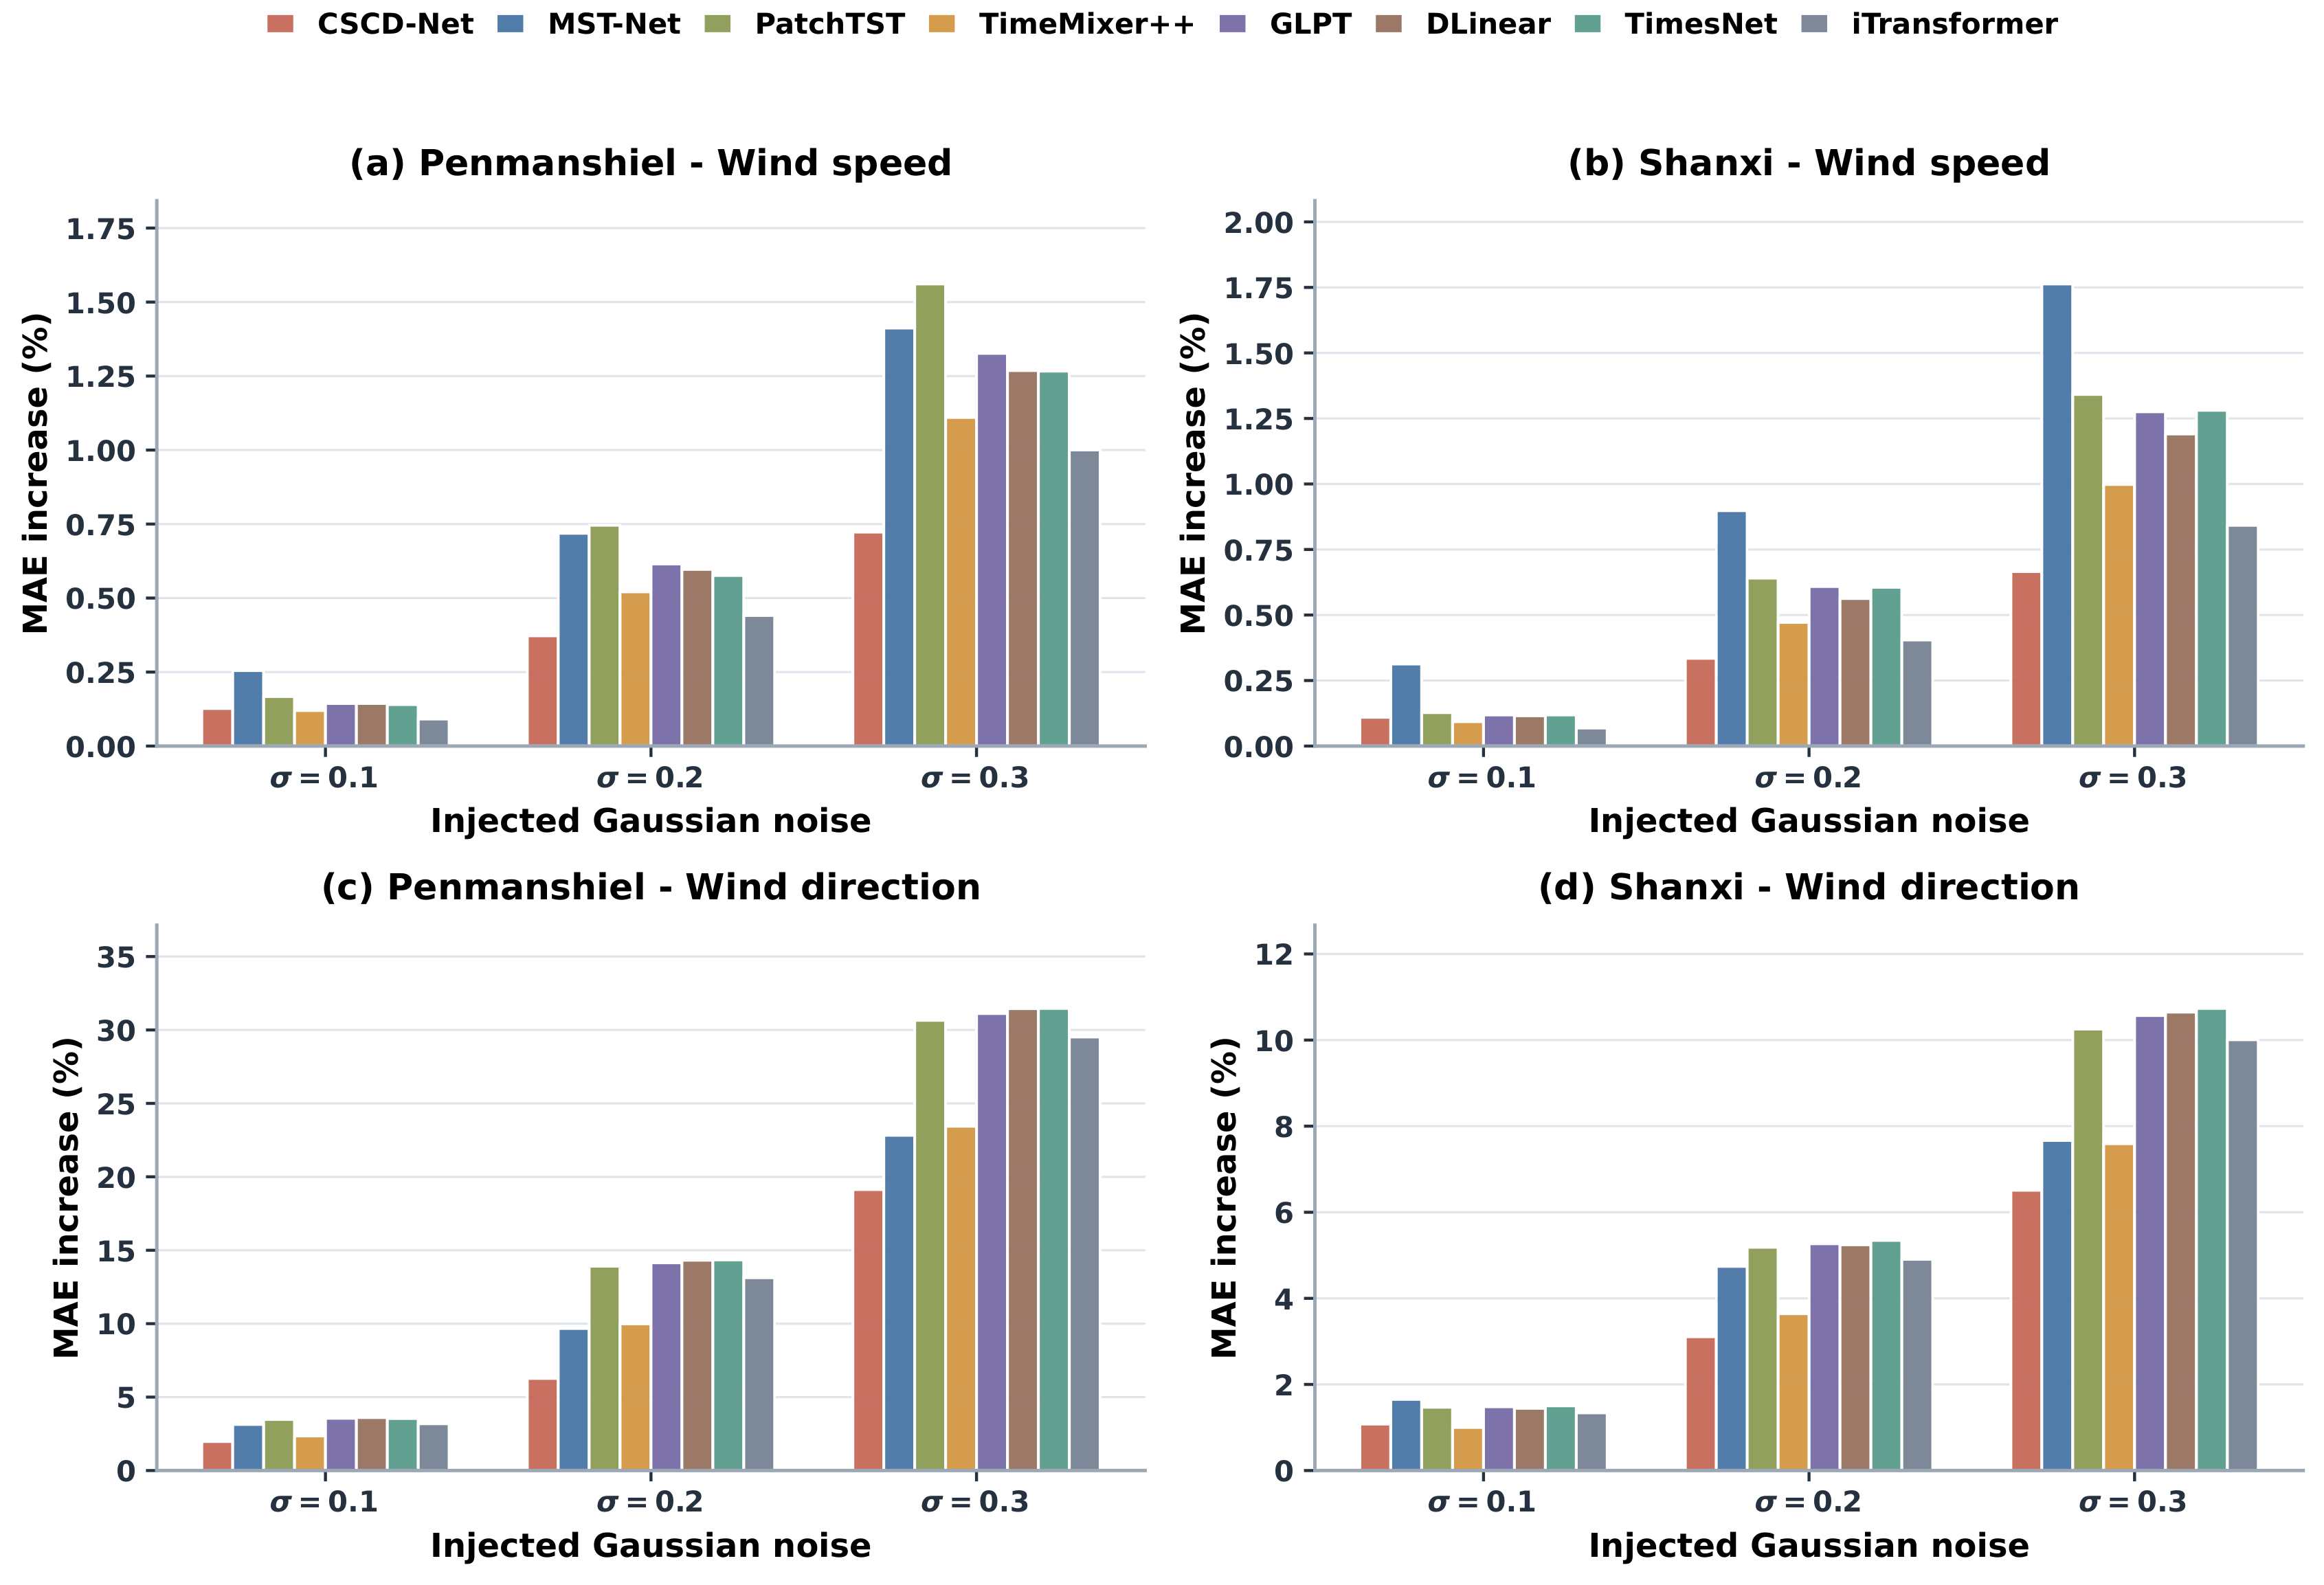
\includegraphics[width=0.48\textwidth]{figures/supp_sensor_robustness.png}
\caption{Sensor Perturbation Robustness. The comparison covers all models, both wind speed and wind direction, and both datasets. Each subplot uses its own vertical scale to preserve dataset-specific variation.}
\label{fig:sensor_perturbation}
\end{figure}

The second experiment evaluates gust-like transient fluctuations through an EVT-inspired residual stratification scheme \cite{Pickands1975StatisticalInferenceUsingExtremeOrderStatistics,Cleveland1990STLSeasonalTrendDecomposition}. For a target series $y_t$, seasonal-trend decomposition using LOESS gives
\begin{equation}
y_t=T_t+S_t+R_t,
\end{equation}
where $T_t$, $S_t$, and $R_t$ denote the trend, seasonal, and residual terms, respectively. The extreme threshold is estimated only from the training split:
\begin{equation}
u=Q_{0.99}\left(\{|R_t|:t\in\mathcal{T}_{\mathrm{train}}\}\right),
\end{equation}
where $Q_{0.99}(\cdot)$ is the 99th percentile. A time step is identified as an extreme event when
\begin{equation}
I_t=\mathbb{I}(|R_t|>u).
\end{equation}
Given an input window of length $L=288$ ending at time $t$, the volatility severity of the corresponding forecasting sample is quantified by
\begin{equation}
N_{\mathrm{extreme}}(t)=\sum_{\tau=t-L+1}^{t}I_{\tau}.
\end{equation}
Test samples are binned by $N_{\mathrm{extreme}}(t)$ and evaluated with the trained model held fixed.

\begin{figure}[!t]
\centering
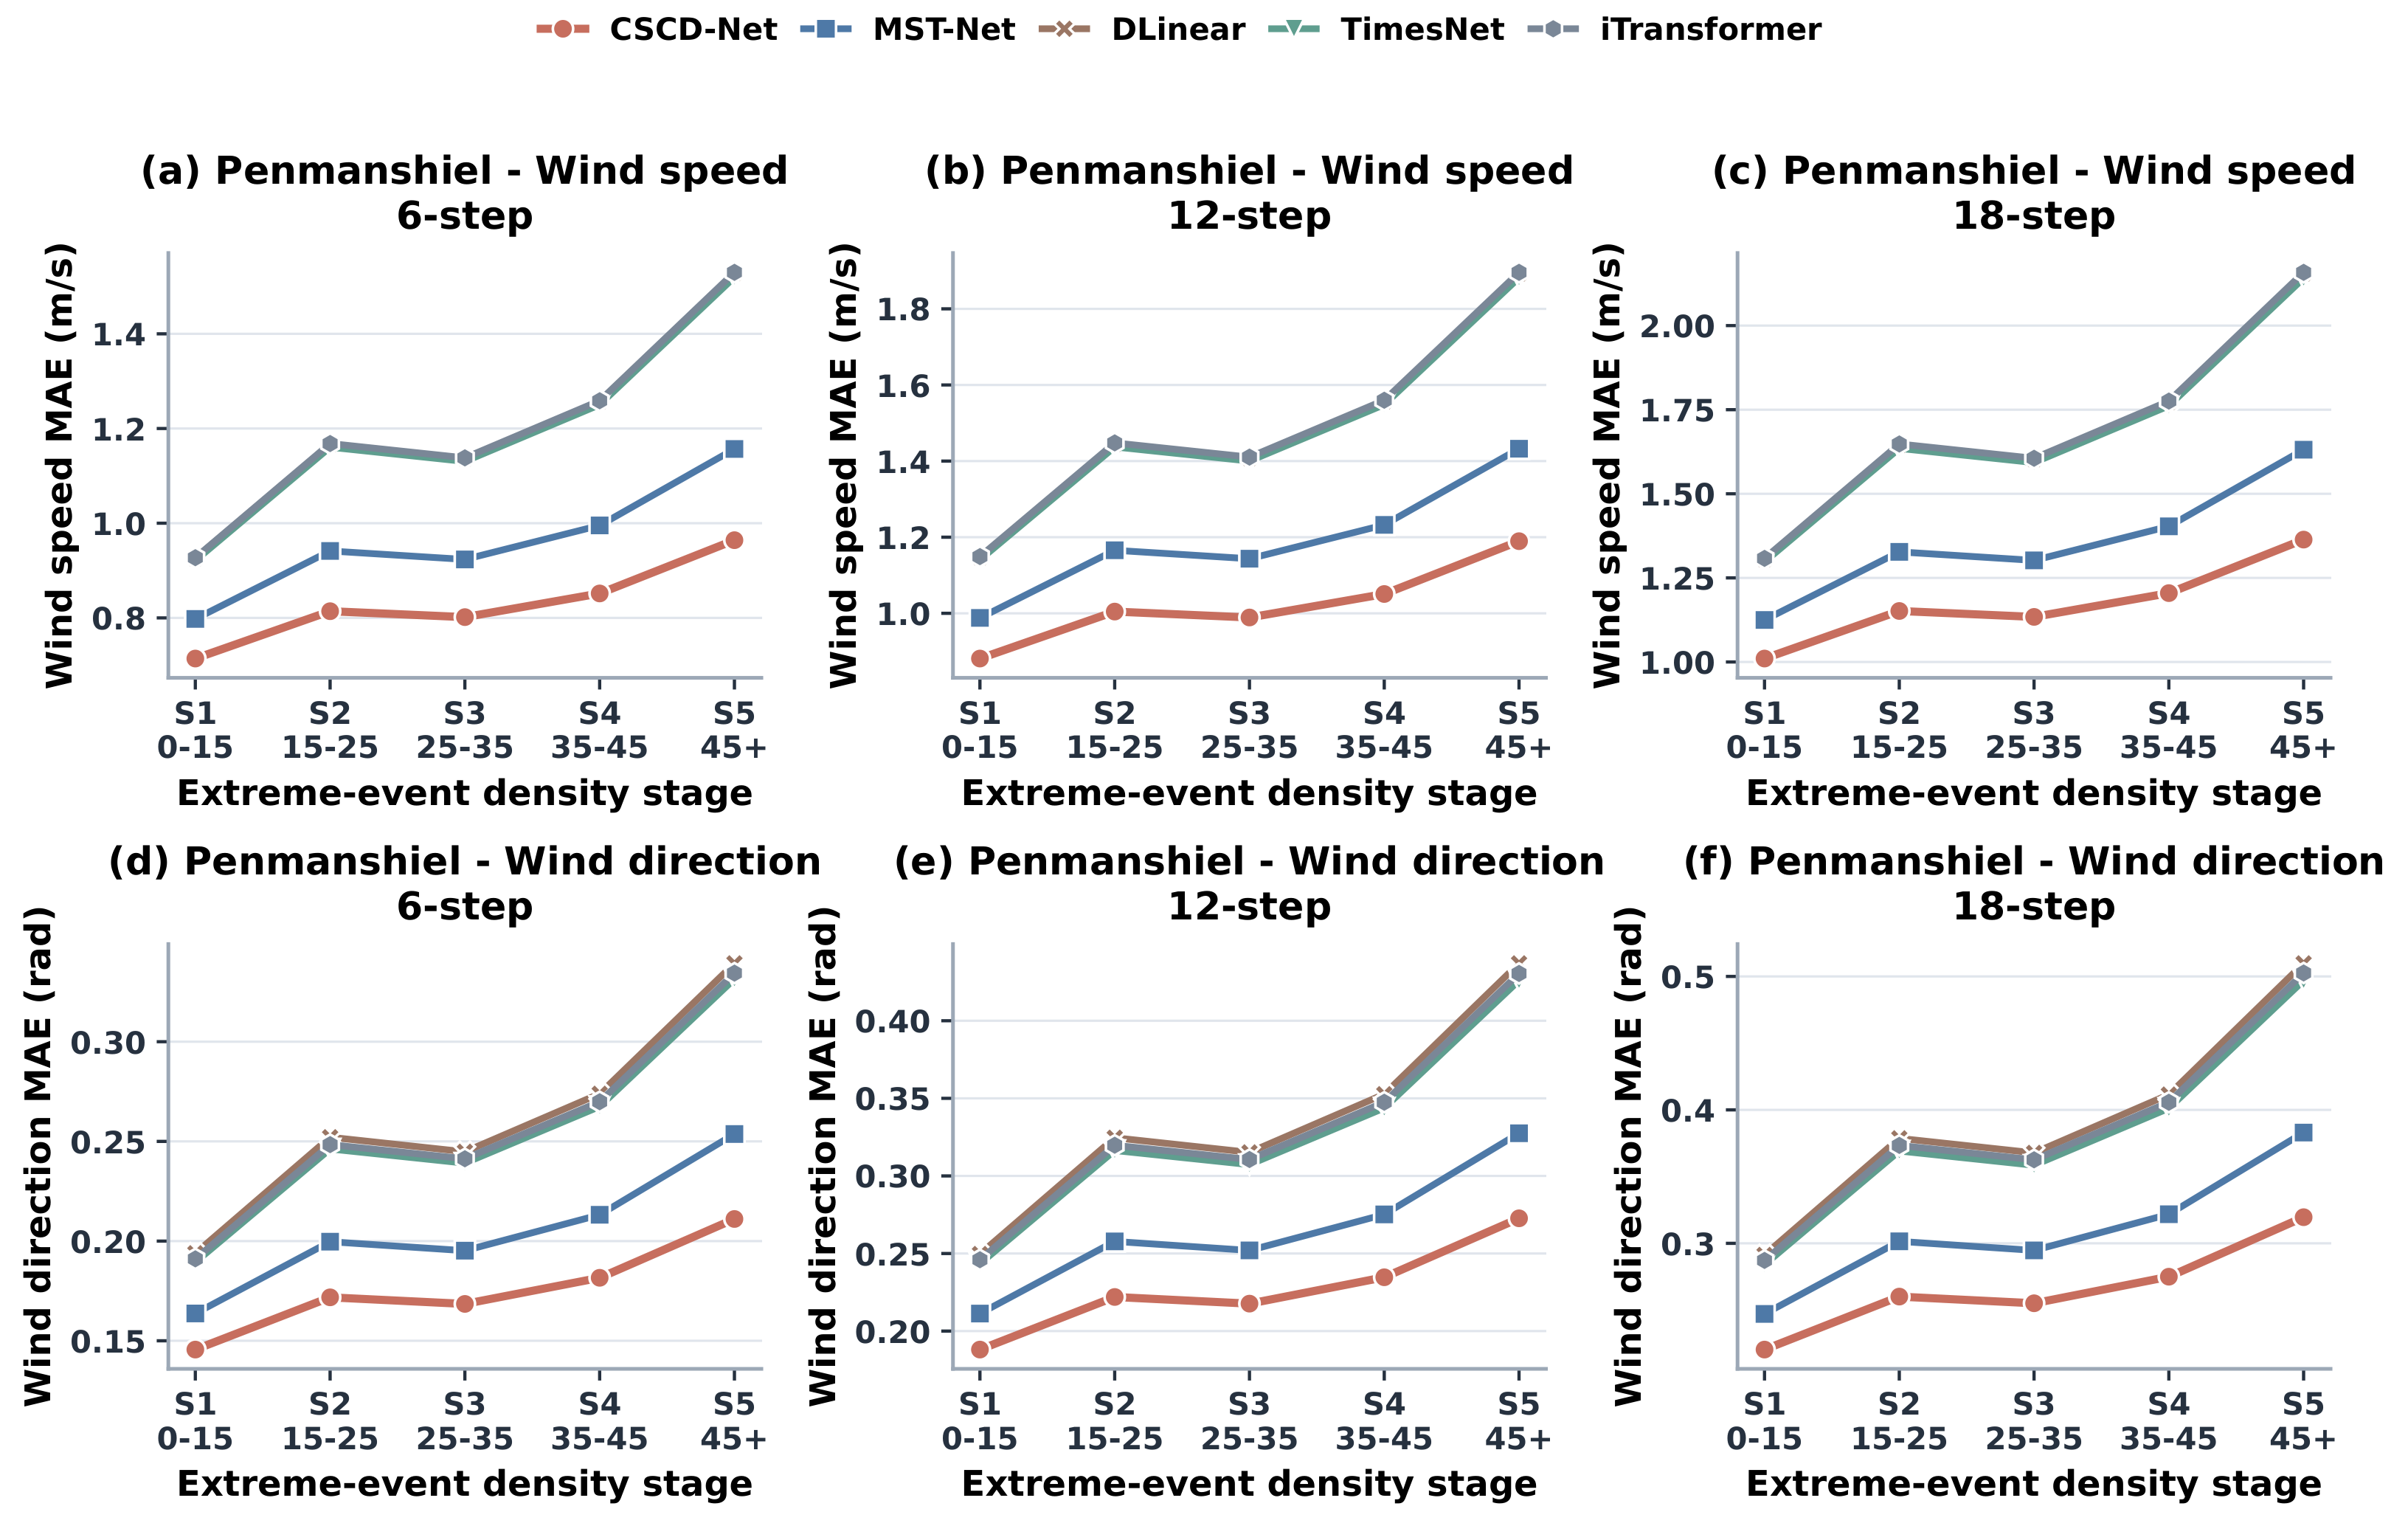
\includegraphics[width=0.48\textwidth]{figures/supp_extreme_stress.png}
\caption{Extreme Volatility Stress Test on the Penmanshiel dataset. The figure reports wind speed and wind direction errors under increasing values of $N_{\mathrm{extreme}}$.}
\label{fig:extreme_stress}
\end{figure}

Figs.~\ref{fig:sensor_perturbation} and \ref{fig:extreme_stress} show that WindFormer yields the smallest degradation under both sensor noise and increasing extreme residual severity.

\subsection{Sparse Deployment Zero-Shot Evaluation}
\label{subsec:zero_shot}

We conduct the \emph{Sparse Deployment Zero-Shot Evaluation} on Penmanshiel. Let $\mathcal{V}$ denote all turbines and $\mathcal{S}_k\subset\mathcal{V}$ the four turbines randomly selected in trial $k$. The remaining turbines
\begin{equation}
\mathcal{U}_k=\mathcal{V}\setminus\mathcal{S}_k
\end{equation}
are treated as unseen zero-shot targets. For a model $f_{\phi}$, $\phi$ is trained only on $\mathcal{D}_{\mathrm{train}}(\mathcal{S}_k)$ and evaluated on $\mathcal{D}_{\mathrm{test}}(\mathcal{U}_k)$. The reported error is averaged over three independent trials:
\begin{equation}
\mathrm{Err}_{\mathrm{ZS}}=\frac{1}{3}\sum_{k=1}^{3}\mathrm{Err}\left(f_{\phi_k},\mathcal{D}_{\mathrm{test}}(\mathcal{U}_k)\right).
\end{equation}
Three conditions are compared: full-sample training, zero-shot transfer, and zero-shot transfer with 0.3-rad angular noise.

\begin{figure}[!t]
\centering
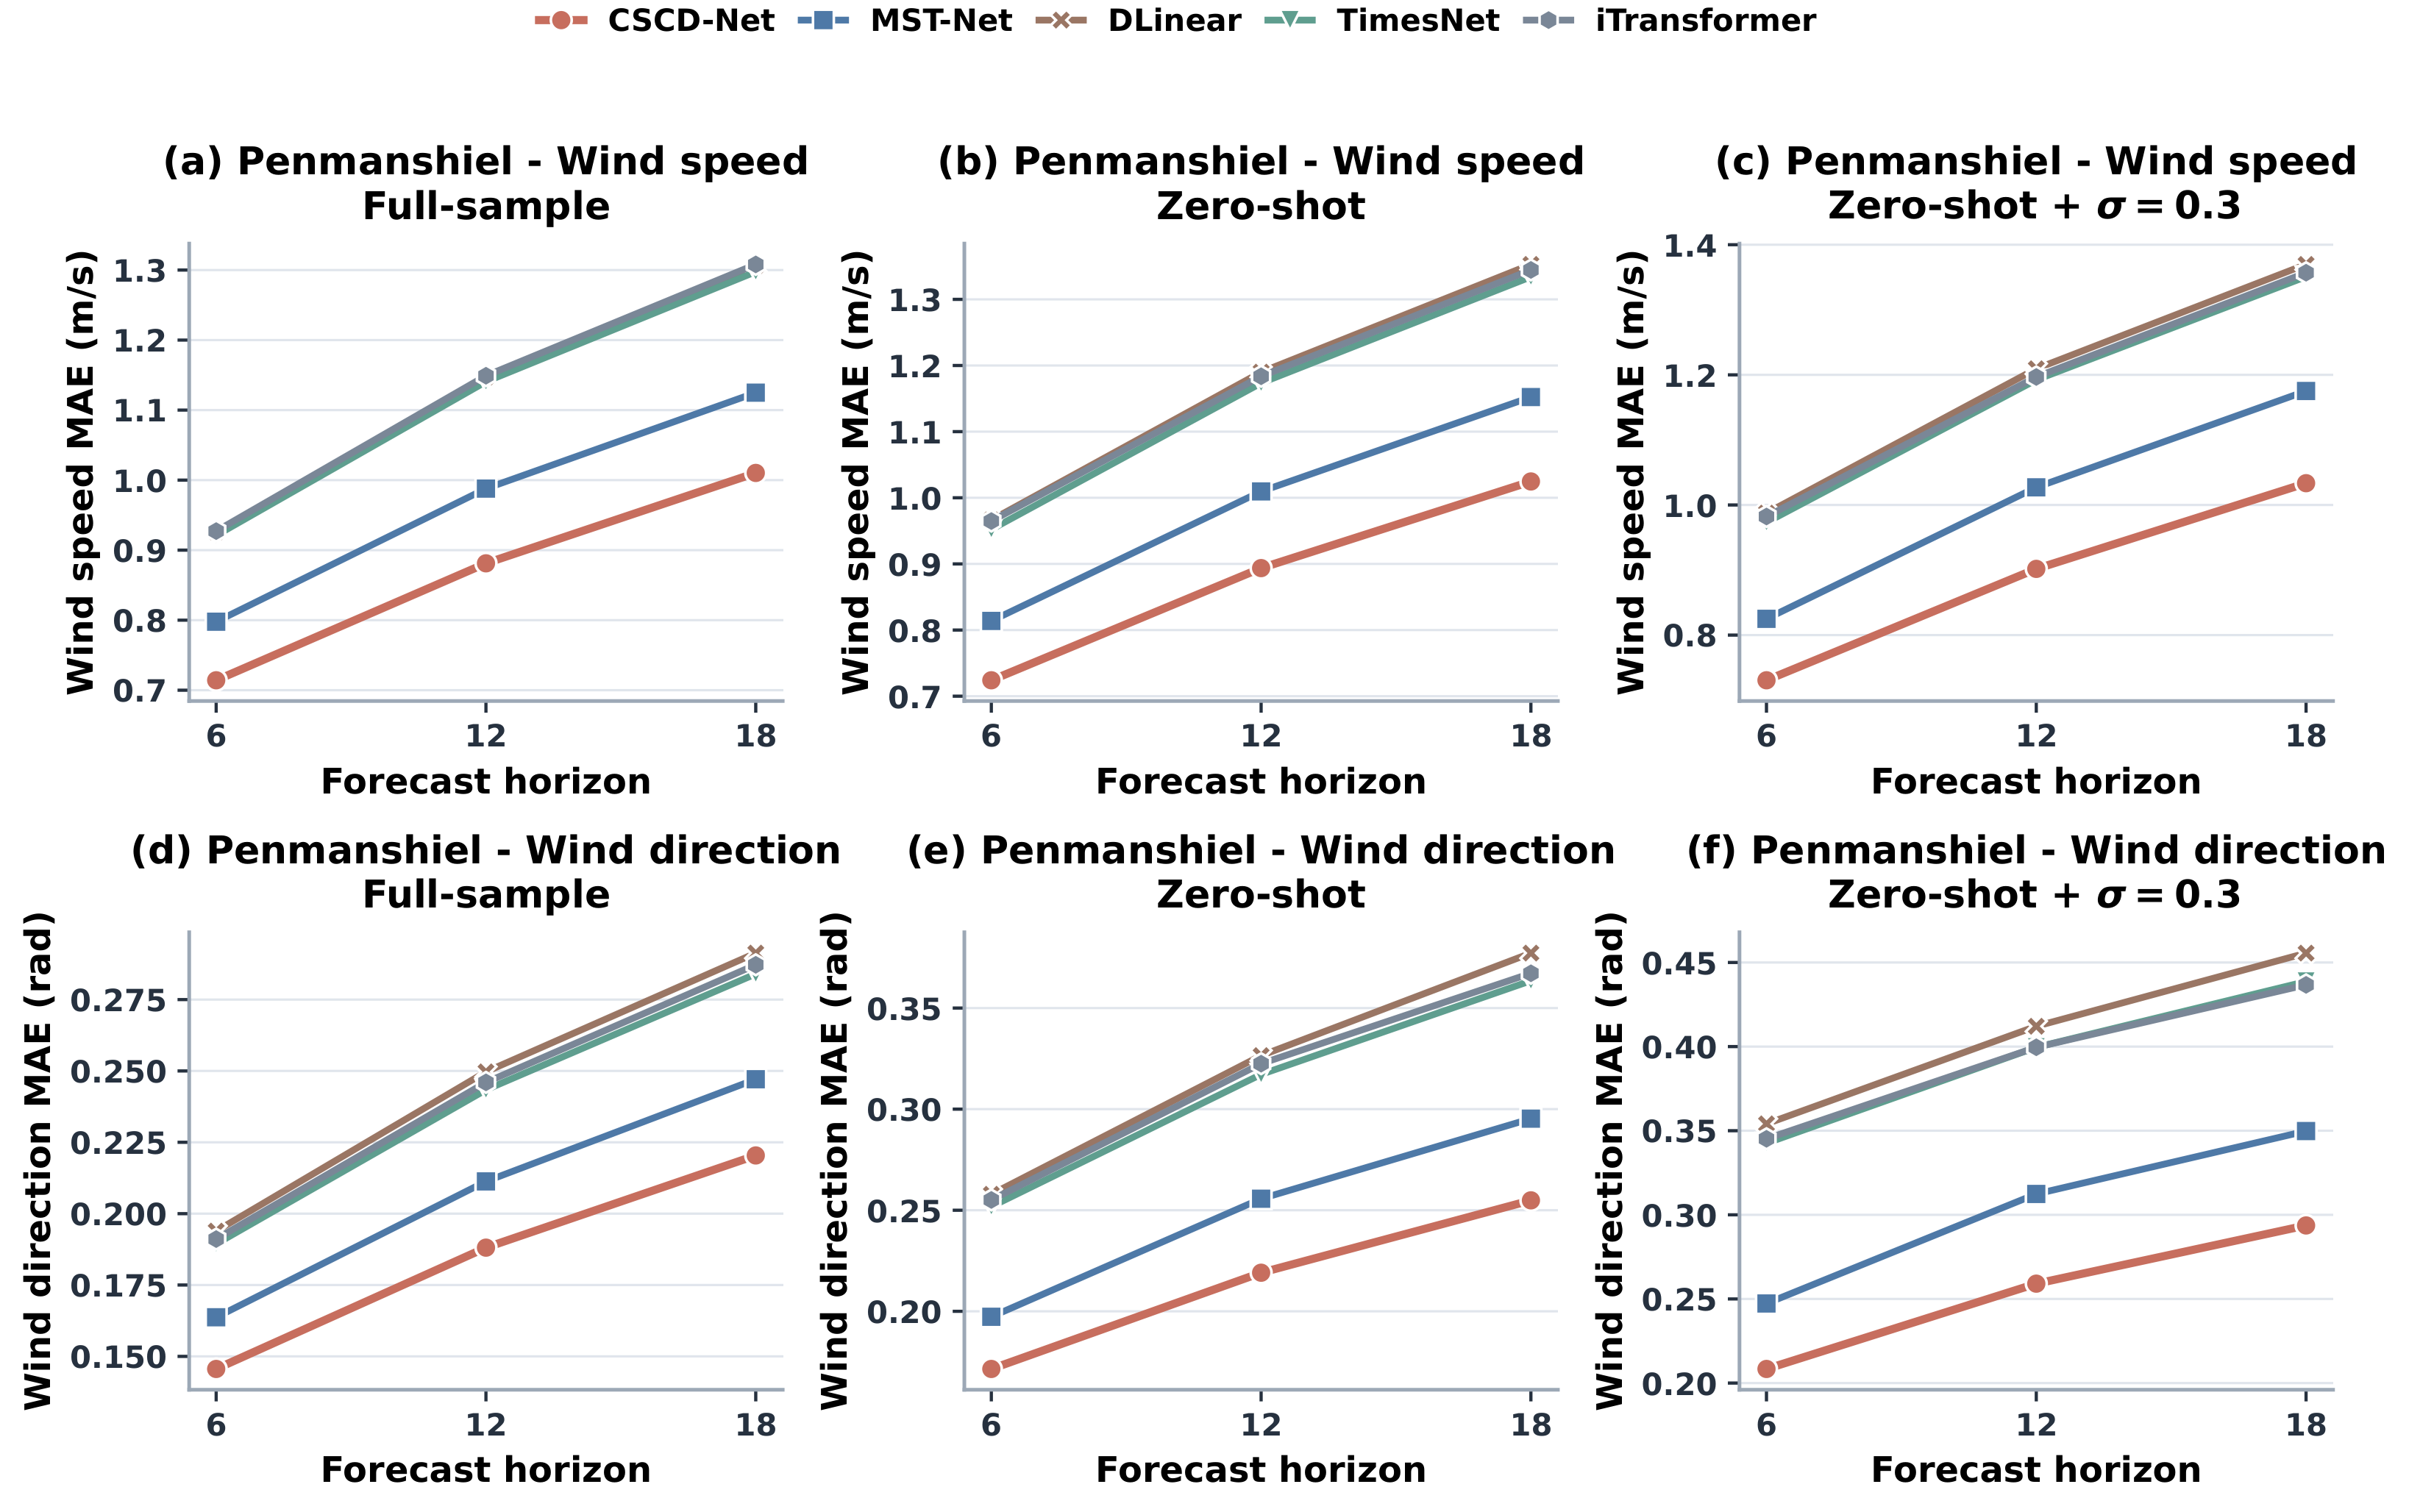
\includegraphics[width=0.48\textwidth]{figures/supp_sparse_zero_shot.png}
\caption{Sparse Deployment Zero-Shot Evaluation on Penmanshiel. The figure compares full-sample training, zero-shot transfer, and zero-shot transfer under sensor noise across multiple forecast horizons.}
\label{fig:sparse_zero_shot}
\end{figure}

Fig.~\ref{fig:sparse_zero_shot} shows that WindFormer has the smallest zero-shot degradation, with a 17.72\% increase in direction MAE under the clean setting and a 15.61\% increase under 0.3-rad noise.

\subsection{Ablation Analysis}
\label{subsec:ablation}

\begin{table*}[!t]
\caption{Ablation study results for different variants on the Shanxi and Penmanshiel datasets.}
\label{tab:ablation}
\centering
\scriptsize
\setlength{\tabcolsep}{3.2pt}
\renewcommand{\arraystretch}{1.08}
\begin{adjustbox}{max width=\textwidth}
\begin{tabular}{l|cccc|cccc|cccc|cccc}
\toprule
\multirow{3}{*}{Variant}
& \multicolumn{4}{c|}{Shanxi-6steps}
& \multicolumn{4}{c|}{Shanxi-12steps}
& \multicolumn{4}{c|}{Penmanshiel-6steps}
& \multicolumn{4}{c}{Penmanshiel-12steps} \\
\cline{2-17}
& \multicolumn{2}{c}{Speed} & \multicolumn{2}{c|}{Wdir}
& \multicolumn{2}{c}{Speed} & \multicolumn{2}{c|}{Wdir}
& \multicolumn{2}{c}{Speed} & \multicolumn{2}{c|}{Wdir}
& \multicolumn{2}{c}{Speed} & \multicolumn{2}{c}{Wdir} \\
\cline{2-17}
& MAE & RMSE & MAE & RMSE
& MAE & RMSE & MAE & RMSE
& MAE & RMSE & MAE & RMSE
& MAE & RMSE & MAE & RMSE \\
\midrule
WindFormer
& \textbf{0.6367} & \textbf{0.9884} & \textbf{0.2717} & \textbf{0.5530}
& \textbf{0.8025} & \textbf{1.2374} & \textbf{0.3441} & \textbf{0.6525}
& \textbf{0.7142} & \textbf{1.1497} & \textbf{0.1456} & \textbf{0.2914}
& \textbf{0.8812} & \textbf{1.4211} & \textbf{0.1881} & \textbf{0.3686} \\
w/o Learnable Weights
& 0.6754 & 1.0421 & 0.2765 & 0.5601
& 0.8465 & 1.3012 & 0.3495 & 0.6612
& 0.7589 & 1.2185 & 0.1502 & 0.2985
& 0.9325 & 1.5052 & 0.1935 & 0.3768 \\
w/o Direction Vector Rep.
& 0.6502 & 1.0065 & 0.6214 & 1.0851
& 0.8188 & 1.2615 & 0.7245 & 1.2562
& 0.7285 & 1.1712 & 0.4985 & 0.8124
& 0.8985 & 1.4485 & 0.5642 & 0.9351 \\
w/o Wind Vector Cons.
& 0.6612 & 1.0215 & 0.2985 & 0.5921
& 0.8315 & 1.2825 & 0.3852 & 0.7124
& 0.7412 & 1.1921 & 0.1685 & 0.3341
& 0.9125 & 1.4721 & 0.2185 & 0.4215 \\
Phase-Attn to Patch
& 0.6845 & 1.0563 & 0.2798 & 0.5644
& 0.8582 & 1.3155 & 0.3541 & 0.6658
& 0.7695 & 1.2312 & 0.1534 & 0.3018
& 0.9458 & 1.5215 & 0.1972 & 0.3812 \\
\bottomrule
\end{tabular}
\end{adjustbox}
\end{table*}

Table~\ref{tab:ablation} validates the contribution of each module. Removing the two-dimensional sine-cosine unit-vector representation mainly harms direction prediction, whereas removing the learnable common-wind weights or replacing Phase-Attention with ordinary patches affects wind-speed prediction more strongly.
